\documentclass[../main.tex]{subfiles}
\begin{document}
\chapter{Certificazione di servizi cloud: il framework CUMULUS}

Come illustrato nel primo capitolo, le tecnologie \textit{cloud} offrono un approccio molto robusto per la fornitura di servizi a livello di infrastruttura, piattaforma e software, alleggerendo in modo considerevole i costi di gestione e manutenzione di infrastrutture computazionali complesse.
Nonostante i benefici economici offerti, il cloud computing pone ancora notevoli problematiche riguardanti sicurezza, privacy, autorità e conformità riguardo ai dati e ai servizi software offerti tramite di esso.
Questi problemi derivano principalmente dalla difficoltà di garantire il mantenimento delle proprietà di sicurezza in un ambiente eterogeneo. Per questo motivo, i fornitori di servizio, rifiutano di assumersi la piena responsabilità sulla sicurezza dei servizi offerti tramite questa tecnologia.
Molti utenti cloud, a partire dalle istituzioni, vorrebbero poter usufruire di servizi \textit{cloud} certificati dal punto di vista della sicurezza.
Sulla base di ciò, si cercherà quindi di definire un framework adatto alla validazione e alla certificazione di infrastrutture, piattaforme e applicativi cloud.
Il progetto in cui si inserisce questo lavoro di tesi è il progetto europeo FP7 CUMULUS (Certification infrastrUcture for MUlti-layer cloUd Services), il quale propone modelli, processi e strumenti al fine di supportare il processo di certificazione per proprietà di sicurezza e non-funzionali in ambito di cloud computing.

\section{Panoramica}
CUMULUS affronta le problematiche descritte tramite lo sviluppo di un framework integrato per la certificazione di applicazioni \textit{cloud} nei tre modelli di servizio (\textit{IaaS}, \textit{PaaS}, \textit{SaaS}), fornendo strumenti di collaborazione tra utenti, fornitori del servizio ospitato sull'infrastruttura \textit{cloud} ed erogatori del servizio \textit{cloud} per assicurare la validità dei certificati di sicurezza in modo continuativo \cite{SpanoudakisDamiani}.

Al fine di effettuare l'\textit{assessment} di determinate proprietà di sicurezza potrebbe essere necessario considerare numerosi tipi di \textit{evidence} catturate a diversi livelli. Queste, affinché possano essere utili per supportare il processo di certificazione, devono essere sanitizzate, aggregate e combinate in modo opportuno.
Affinché sia possibile porre fiducia sul livello hardware, è possibile utilizzare la \textit{Trusted Computing Platform}, che può fornire la prova che il sistema che si sta ri-certificando sia lo stesso sul quale la certificazione è stata effettuata la prima volta. 
Ad esempio, una certificazione per l'integrità dei dati dovrebbe considerare sia la possibilità di modifica e corruzione da parte di un software che una manomissione dei dati a livello hardware (ad esempio tramite il collegamento del dispositivo di memorizzazione ad un'altra macchina o l'uso di strumenti specifici per bypassare i controlli di sicurezza del file system).
Per ottenere ciò si possono utilizzare strumenti specifici come il TPM (\textit{Trusted Platform Module}), che effettua la firma e i controlli di integrità delle informazioni sensibili con chiavi memorizzate in hardware.
L'integrazione di evidenze eterogenee ottenute dal testing di differenti livelli permettono di definire CUMULUS un framework \textit{multi-layer}.
Viene quindi introdotto il concetto di \textit{certificazione ibrida}: certificati basati sul collaudo su del software effettuato in un ambiente caratterizzato da determinate condizioni, possono essere combinati con i risultati di operazioni di monitoraggio nel momento in cui le condizioni originali decadono.\cite{SpanoudakisDamiani}

Visti gli oneri e i costi implicati da un processo complesso come quello della certificazione, lo schema ivi descritto propone:
\begin{itemize}
\item Un processo di certificazione iniziale di tutte le proprietà non funzionali e di sicurezza, di costo $c_1$
\item Più processi di certificazione incrementali, aventi costo $c2 \sim\frac{c1}{n}$, eseguito ad ogni cambiamento del modello di certificazione o di un \textit{asset} critico per la proprietà di sicurezza associata.
\end{itemize}
La certificazione incrementale può essere supportata dal monitoraggio continuativo del servizio cloud, anziché dall'utilizzo continuativo di tecniche statiche come il testing \cite{Dempsey}.%K. Dempsey et al., “Information Security Continuous Monitoring (ISCM) for Federal Systems and Organisations,” NIST 800-137, 2011

\section{Il processo di certificazione}

Affinché sia possibile certificare un servizio cloud è necessario strutturare un processo di certificazione improntato sulla collaborazione di diverse parti\cite{Cloud1}:
\begin{itemize}
\item Un \textit{Fornitore del servizio}, che ha sviluppato il servizio cloud da certificare.
\item Un \textit{Fornitore del servizio cloud}, che fornisce l'accesso alle funzionalità di backend per supportare il processo di certificazione.
\item Una \textit{Certification Authority}, che amministra e gestisce il processo di certificazione.
\item Uno o più \textit{Accredited lab}, a cui è delegata la responsabilità della valutazione del sistema cloud. Può essere sia un attore specifico, che utilizza il framework per l'emissione del certificato, che un ulteriore framework che esegue automaticamente i processi di certificazione e la verifica dei certificati precedentemente emessi seguendo le linee guida della \textit{Certification Authority}.
\end{itemize}

L'obiettivo del processo di certificazione è quello di produrre e mantenere un certificato  di sicurezza per un sistema \textit{target} (\textit{ToC, Target of Certification}), comprendente tutte le evidenze a supporto delle proprietà certificate.\cite{Cloud1}
Differentemente da i processi di certificazioni tradizionali per i software e i servizi SOA, il processo di certificazione per servizi cloud proposto è composto da due fasi:
\begin{enumerate}
\item \textit{Pre-deployment evaluation}, una fase preliminare nella quale l'\textit{Accredited lab} effettua una valutazione statica del \textit{ToC} in un ambiente di laboratorio e colleziona le evidenze a supporto delll'emissione del certificato
\item \textit{In-production evaluation}, nella quale viene effettuato il controllo continuativo della validità del certificato all'interno dell'ambiente di produzione reale.
\end{enumerate}

Nel caso in cui non sia possibile effettuare la fase di \textit{Pre-deployment evaluation} (es. non è possibile fornire un ambiente di laboratorio adatto a certificare un determinato prodotto per una determinata proprietà), la raccolta delle evidenze viene fatta durante la fase di produzione.
Quando invece è la fase di \textit{In-production evaluation} a non poter essere eseguita (ad esempio nel caso di un test di robustezza contro un attacco di tipo DDoS\footnote{Distributed denial of service}, che potrebbe causare un'interruzione del servizio), viene emesso un certificato statico durante la fase preliminare e non viene effettuata alcuna verifica continuativa della validità della proprietà.\cite{Cloud1}

Come discusso nel documento \cite{TrustModelCloudAnisDamArd} il processo di certificazione preso in considerazione è basato su:
\begin{enumerate}
\item una \textit{proprietà di sicurezza} da certificare, definita in modo astratto (es. confidenzialità, integrità, disponibilità), definita utilizzando gli attributi in base ai meccanismi di sicurezza implicati o ai possibili attacchi;
\item un \textit{target di certificazione}, o \textit{ToC}, che definisce il perimetro della certificazione come un insieme di meccanismi appartenenti ad uno o più livelli dello stack cloud;
\item una descrizione delle attività di valutazione, espresse come un insieme di configurazioni possibili per la validazione della proprietà da certificare;
\item le \textit{evidenze} a supporto del certificato emesso nei confronti del \textit{ToC}.
\end{enumerate}

Questi elementi sono una parte di documenti più generali che costituiscono gli input e gli output del processo di certificazione.
Gli input del  processo di certificazione sono:\cite{TrustModelCloudAnisDamArd}
\begin{itemize}
\item \textit{Certification Model (CM) Template}: è una rappresentazione astratta degli input del processo di certificazione, che specifica le configurazioni e le attività della certificazione di una determinata proprietà per una determinata classe di ToC con un alto livello di astrazione. Viene firmato dalla \textit{Certification Authority}.
\`E composto dai seguenti elementi:
\begin{itemize}
\item \textit{ToC} - descrive il servizio/applicazione da certificare, specificandone la classe e il livello cloud di appartenenza
\item \textit{Collectors} - Contiene un insieme di elementi chiamati \textit{AbstractCollectors} e \textit{Collectors} il cui compito è quello di descrivere il processo di collezionamento delle evidenze per una data proprietà e ToC.
I templates specificano solamente gli \textit{AbstractCollectors} che descrivono il modello del flusso alla base del collezionamento delle evidenze. Ogni AbstractCollector descrive le attività senza definire i casi di test reali da eseguire sul ToC ai fini della certificazione. Lo scopo è quello di definire un insieme di flussi (utilizzo di input random, partizionamento degli input) e categorie (funzionali, di robustezza, penetration test) per le determinate tipologie di test.
\item \textit{Signature} - fornisce la firma dell'autorità di certificazione che ha responsabilità sul template. \`E fondamentale per stabilire un rapporto di fiducia nel framework che implementa questo processo.
\end{itemize}
\item \textit{Certification Model (CM) Instance} - è una rifinitura del \textit{Template} che guida in modo effettivo il processo di certificazione. Include le informazioni specifiche sulle configurazioni e sulle attività da eseguire sullo specifico \textit{ToC} da valutare.
\`E composto dai seguenti elementi:
\begin{itemize}
\item \textit{ToC} - specializza il ToC definito nel template definendo
un insieme di elementi ToT (Target of Test). Ogni elemento
ToT fornisce i riferimenti agli endpoint (hooks)
necessari alla valutazione del ToC.
Successivamente guida l'esecuzione dei casi di test tramite le \textit{probe} e il collezionamento dei risultati dell'esecuzione.
\item \textit{Collectors} - estende l'elemento Collectors del Template, con un insieme di elementi Collector e, se necessario, ridefinendo gli Abstract Collector.
Ogno collector è riferito in base a un AbstractCollector e specifica i casi di test reali da eseguire.
\item \textit{Aggregator} - Ogni Collector è associato a un elemento Aggregator che è usato per calcolare lo stato dell'intera attività di test condotta dal Collector stesso.
Lo stato è un valore booleano, dove il successo (1) e il fallimento (0) sono definite come metriche sui risultati dei test prodotti da ogni Collector.
Ad esempio, un Collector può avere successo se una determinata percentuale di casi di test sono stati eseguiti con successo.
\item \textit{LifeCycle} - Descrive il ciclo di vita del certificato. Specifica tutte le condizioni (espressioni booleane) che regolano le transizioni tra gli elementi dell'Aggregator.
\item \textit{Signature} - fornisce la firma del framework di certificazione delegato dalla Certification Authority per la firma del CM Instance.
La firma è necessaria per stabilire una catena di fiducia per i certificati prodotti.
\end{itemize}
\end{itemize}

La consistenza tra il \textit{CM Template} e il \textit{CM Instance} e tra il \textit{CM Instance} e il \textit{ToC} viene effettuata manualmente dall'\textit{accredited lab} durante la fase di valutazione  \textit{pre-deployment}.

L'output del processo di certificazione è costituito dal \textit{certificato}, che contiene tutte le informazioni e i risultati ottenuti dal processo di valutazione, comprese le evidenze a supporto della validità del certificato.

Nella figura \ref{fig:processocertific} è mostrato il framework concettuale alla base del processo di certificazione\cite{TrustModelCloudAnisDamArd}.
Nel momento in cui il fornitore di servizi effettua il \textit{deploy} dell'applicazione sul \textit{cloud} (\textit{ToC}), ingaggia una \textit{Certification Authority} affinché emetta un certificato per un determinato insieme di proprietà, selezionando un \textit{CM Template}.
La \textit{Certification Authority} delega quindi all'\textit{accredited lab} la produzione del \textit{CM instance}.
Se le evidenze prodotte nelle fasi di valutazione \textit{pre-deployment} e \textit{in-production} sono sufficienti, viene quindi emesso (o rinnovato) il certificato, includendo le proprietà certificate, l'identità del ToC e le evidenze a supporto del processo di certificazione.
\begin{figure}[H]
\centering
\makebox[\textwidth]{
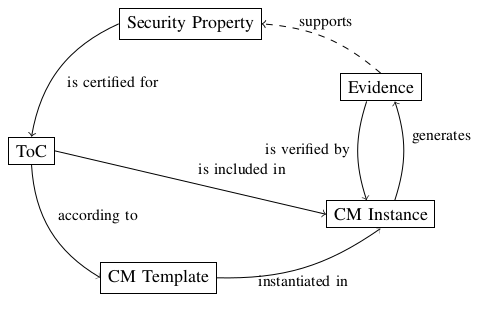
\includegraphics[width=10cm]{immagini/FrameworkCert.png}
}
\caption{Rappresentazione concettuale del framework CUMULUS \cite{Cloud1}}\label{fig:processocertific}
\end{figure}

Nella figura \ref{fig:lifecyclecertificato} è mostrato invece il ciclo di vita di un certificato, dalla sua emissione fino alla sua scadenza o revoca.
Esso è modellato secondo un automa a stati finiti, dove ogni vertice è uno stato (\textit{not issued}, \textit{issued}, \textit{suspended}, \textit{revoked}, \textit{expired}) e ogni arco è una transizione tra i due stati, regolata da una condizione dipendente da un'evidenza collezionata.
\begin{figure}[H]
\centering
\makebox[\textwidth]{
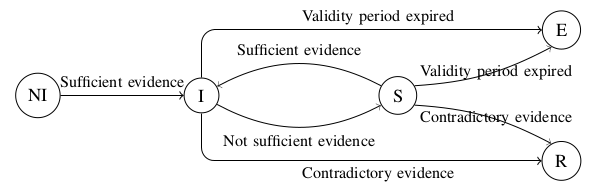
\includegraphics[width=10cm]{immagini/LifeCycle.png}
}
\caption{Ciclo di vita del certificato \cite{Cloud1}}\label{fig:lifecyclecertificato}
\end{figure}


\section{Requisiti del framework di certificazione}

I requisiti del framework per la certificazione di sicurezza per servizio cloud sono i seguenti:\cite{Cloud1}
\begin{enumerate}
\item \textit{Distributed deployment}: \textbf{deve} fornire la possibilità di effettuare il deployment distribuito dei componenti.
\item \textit{Multi-Layer and Multi-Tenant certification}: \textbf{dovrebbe} essere in grado di certificare le  proprietà di sicurezza dei servizi e delle applicazioni che spaziano su diversi livelli dello stack \textit{cloud} (dal livello applicativo al livello di infrastruttura). Per esempio la confidenzialità dei dati trasmessi e memorizzati da un'applicazione,  è una proprietà che dipende dai meccanismi implementati a tutti i livelli dello stack cloud.
\item \textit{Property-driven certification}: \textbf{dovrebbe} implementare un processo di certificazione guidato dalla specifica proprietà da certificare sul sistema target.
\item \textit{Evidence-based certification}: \textbf{deve} supportare un processo di certificazione che produca un insieme di evidenze sufficienti a dimostrare la proprietà di sicurezza certificata e le includa nel certificato emesso. Le evidenze \textbf{dovrebbero} essere collezionate in modo standard dagli agenti e dalle sonde deployate nel sistema da certificare, in base al meccanismo utilizzato.
\item \textit{Incremental certification}: \textbf{dovrebbe} fornire un approccio continuativo e incrementale, mediante la ri-valutazione runtime delle evidenze e dei certificati. 
\item \textit{Fully Automatic Configuration}: \textbf{potrebbe} garantire un processo automatico per il \textit{deployment} e la configurazione degli agenti e delle sonde, supportando il collezionamento e l'esecuzione di processi di certificazione in modo automatico, anche per la certificazione incrementale.
\item \textit{Extendible deployment}: \textbf{deve} essere personalizzabile e adattabile ai requisiti di un servizio in continua evoluzione.
\item \textit{Trusted implementation}: \textbf{deve} essere affidabile e deve garantire l'affidabilità di tutte le attività da esso svolte, affinché sia possibile aumentare la consapevolezza della correttezza del processo svolto da parte dell'utente.
\end{enumerate}
Inoltre, si vuole dare la possibilità a sviluppatori, architetti, ingegneri, sistemisti e sviluppatori di progettare infrastrutture, piattaforme e software che siano in grado di supportare il processo di certificazione.
Dei requisiti aggiuntivi per soddisfare questo obiettivo possono essere:
\begin{enumerate}
\item \textit{Certification-aware cloud engineering}: \textbf{dovrebbe} fornire un approccio orientato alla certificazione facilmente integrabile con le metodologie di sviluppo  tradizionali. In questa maniera viene facilitata la generazione dei test già nella fase di \textit{development} di un'applicazione.
\item \textit{Guided security mechanism development}: \textbf{deve} guidare lo sviluppo dei meccanismi di sicurezza necessari alla certificazione di un sistema per una determinata proprietà.
\item \textit{Step-by-step Deployment}: \textbf{deve} guidare il deployment di tutti i componenti necessari per supportare l'esecuzione del processo di certificazione.
\item \textit{Certification process independent}: \textbf{dovrebbe} implementare una metodologia per l'ingegnerizzazione delle infrastrutture cloud orientata alla certificazione ma completamente indipendente dallo specifico processo di certificazione.
\end{enumerate}

\section{Componenti e architettura del framework}
L'architettura del framework CUMULUS è mostrata in figura \ref{figInfrastruct}. Essa comprende \cite{SpanoudakisDamiani}:
\begin{itemize}
\item Security Models e Certification Models
\item Componenti per la produzione dei test, per il monitoraggio, per la certificazione basata sul trusted computing, per la certificazione incrementale e per la certificazione ibrida
\item Componenti per la raccolta di evidenze a supporto del processo di certificazione
\item Un protocollo di interazione per la raccolta delle evidenze
\item Strumenti a supporto dell'ingegnerizzazione dei servizi da certificare
\end{itemize}

\begin{figure}[H]
\centering
\makebox[\textwidth]{
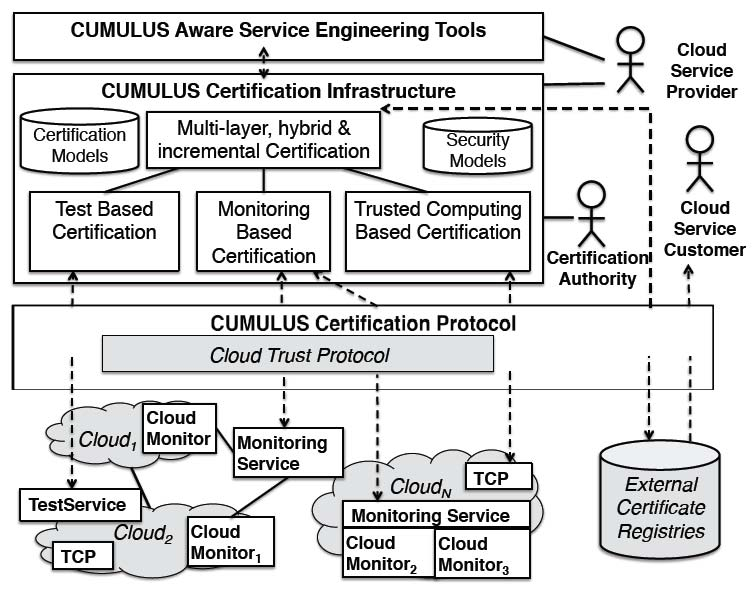
\includegraphics[width=13cm]{immagini/CumulusStructure.png}
}
\caption{Architettura del framework CUMULUS \cite{SpanoudakisDamiani}}\label{figInfrastruct}
\end{figure}

Il framework è organizzato secondo un'architettura master/slave composta dall'interazione di due moduli principali\cite{Cloud1}:
\begin{itemize}
\item \textit{Test Manager} - master - è il componente software che gestisce tutto il processo di certificazione. Esso:
\begin{enumerate}
\item Fornisce un'interfaccia esterna per la gestione del processo di certificazione (start, stop, restart etc.) e per amministrare, ottenere e modificare i relativi \textit{CM instances} e i certificati emessi
\item Elabora i \textit{CM Instances} per estrarre le configurazioni e i casi di test necessari all'esecuzione del processo di certificazione e per l'inizializzazione dei componenti \textit{slave}
\item Amministra il ciclo di vita dei certificati esterni raccogliendo e aggregando i risultati delle attività di test.
\end{enumerate}
\item Più \textit{Test Agent} - slave - che si occupano dell'esecuzione dei test sul \textit{ToC}. Si occupa di:
\begin{enumerate}
\item Installare gli script dei test sulle macchine target (chiamate \textit{ToT, Target of Test}), ottenuti da un repository centralizzato strutturato in modo da garantire l'integrità dei test
\item Eseguire i casi di test specificati
\item Effettuare la raccolta delle evidenze e restituire i risultati delle attività dei test al Test Manager.
\end{enumerate}
\end{itemize}
Il deploy dei Test Agent è automatizzato, al fine di supportare la scalabilità e l'esecuzione di molteplici processi di certificazione in parallelo. Anche il Test Agent offre funzionalità di scalabilità, distribuendo il carico dei singoli script di testing su più processi tramite uno schedulatore. 
Nella figura \ref{fig:InterazTaTm} è mostrata l'interazione tar il \textit{Test Agent} e il \textit{Test Manager}, l'iniezione degli script tramite gli \textit{hooks} e l'esecuzione degli script sul \textit{ToC}.

\begin{figure}[H]
\centering
\makebox[\textwidth]{
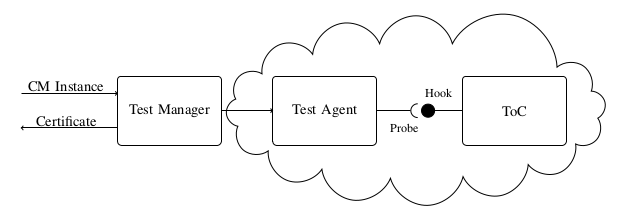
\includegraphics[width=13cm]{immagini/InterazTaTm.png}
}
\caption{Architettura del framework CUMULUS \cite{Cloud1}}\label{fig:InterazTaTm}
\end{figure}

Il processo di certificazione inizia nel  momento in cui  un \textit{CM Instance} viene mandato al Test Manager.
Il Test Manager ne effettua il parsing e, nel caso in cui non siano già presenti, effettua il \textit{deploy} degli agenti necessari e fornisce ad essi le configurazioni per l'esecuzione dei test.
Il Test Agent esegue il test, colleziona le evidenze e restituisce i risultati al Test Manager.
Gli \textit{hooks} sono forniti dal fornitore del servizio e sono generalmente protetti da sistemi di controllo degli accessi.

Nella figura \ref{fig:TMTAComponents} sono mostrati i componenti interni del Test Manager e del Test Agent e la loro interazione.

\begin{figure}[H]
\centering
\makebox[\textwidth]{
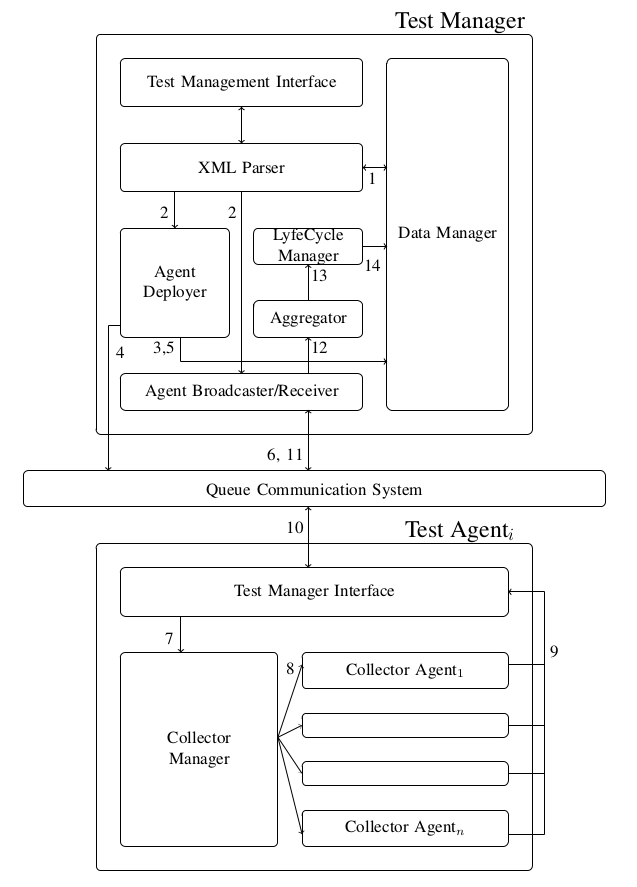
\includegraphics[width=13cm]{immagini/TMTAComponents.png}
}
\caption{Test Manager e Test Agent: componenti interni \cite{Cloud1}}\label{fig:TMTAComponents}
\end{figure}

\subsection{Componenti del Test Manager}
I componenti del TM possono essere raggruppati in tre famiglie:
\begin{enumerate}
\item Componenti di comunicazione (\textit{Test Management Interface, Agent-broadcaster/Receiver, Agent Deployer, Queue Communication System})
\item Componenti di gestione dei dati (\textit{Data Manager})
\item Componenti di engine (\textit{XML Parser, LifeCycle Manager, Aggregator})
\end{enumerate}
\begin{itemize}
\item \textit{Test Management Interface}: front-end del processo di certificazione. Offre delle API per controllare il processo di certificazione, ottenere i certificati e ispezionare il \textit{life cycle}
\item \textit{Data Manager}: gestisce le informazioni persistenti sul Test Manager. Utilizza un database per memorizzare tutti gli \textit{artifacts}, inclusi i \textit{CM instances} ed i certificati ad essi relativi.
\item \textit{XML Parser}: implementa tre funzionalità principali:
\begin{enumerate}
\item effettua il parsing di tutti i documenti utilizzati dalla \textit{Test Management Interface};
\item genera i certificati quando richiesto dalla \textit{Test Management Interface};
\item effettua il parsing del \textit{CM instance} e prepara i comandi da far eseguire al \textit{Test Agent}.
\end{enumerate}
\item \textit{Agent Broadcaster/Receiver}: è responsabile di gestire la comunicazione con gli agenti. \`E anche responsabile di effettuare il \textit{dispatching} dei messaggi provenienti dagli agenti verso gli altri componenti del TM. 
\item \textit{Meccanismo di comunicazione basato su coda}: inoltra i messaggi dagli agenti a un sistema di broadcasting e ricezione. Gestisce anche l'autenticazione degli agenti sulle code di messaggi.
\item \textit{Agent deployer}: interagisce con le APIs cloud (ad esempio le APIs di OpenStack) per effettuare il deploy degli agenti, permette loro di autenticarsi con il Test Manager abilitandoli alla comunicazione e mantiene una lista di tutti gli agenti disponibili per l'esecuzione di test.
\item \textit{Aggregatore}: effettua la valutazione dei risultati dei test effettuati dal Test Agent e invia una notifica al LifeCycle Manager. L'aggregazione avviene in base a metriche specificate nell'elemento \textit{Aggregator} del \textit{CM Instance}.
\item \textit{LifeCycle Manager}: riceve la valutazione effettuata dall'aggregatore e, rispettando le condizioni di transizione specificate nel \textit{LifeCycle}, imposta lo stato del certificato.
\end{itemize}
\subsection{Componenti del Test Agent}
I compnenti del Test Agent sono i seguenti:
\begin{itemize}
\item \textit{Test Manager Interface}: riceve i comandi dal Test Manager e
restituisce i risultati dei test al Test Manager
\item \textit{Collector Manager} Amministra l'installazione, la configurazione e l'esecuzione dei test, effettuando la raccolta delle evidenze e raccogliendo informazioni nei \textit{log} per eventuali operazioni di auditing successive e analisi a posteriori.
\item \textit{Collector Agent} \`E il singolo processo di testing, avviato alla ricezione di un Test Case in parallelo.
\end{itemize}

\subsection{Flusso di esecuzione}
Il flusso di esecuzione del processo di certificazione è mostrato nella figura \ref{fig:TMTAComponents} e si articola come segue:
\begin{enumerate}
\item Il Data Manager estrae il CM Instance dal database
\item L'XML Parser effettua il parsing per generare le informazioni da inviare al Test Agent
\item L'XML Parser estrae tutte le informazioni necessarie all'eventuale deployment del Test Agent e all'esecuzione del test
\item L'Agent Deployer controlla i Test Agent registrati, alla ricerca di un Test Agent adatto ad avviare il processo di testing. Se non trova un Test Agent idoneo, ne effettua il deploy e lo registra.
\item Una volta che il Test Agent è pronto, gli vengono inviate tutte le informazioni tramite l'Agent Broadcaster/Receiver.
\item Il Test Agent effettua il parsing tramite il Collector Manager
\item Ogni Collector Agent viene lanciato in parallelo e avvia tutti i Test Cases appartenenti al Collector ricevuto.
\item Ogni risultato viene inviato  al Test Manager tramite la Test Manager Interface
\item L'Agent Broadcaster/Receiver riceve il messaggio e lo inoltra all'aggregatore che ha tutte le informazioni necessarie per effettuare la valutazione del collector.
\item L'Aggregatore notifica il LifeCycle Manager che effettua la valutazione delle transazioni, aggiornando eventualmente lo stato del certificato.
\end{enumerate}

\section{Strategie di deployment}
Il deployment di questo framework potrebbe essre considerato invasivo dai fornitori di servizi, che dovrebbero aprire i propri sistemi ad agenti di test di terze parti.
Inoltre i CM Instance potrebbero contener informazioni con un alto livello di confidenzialità come configurazioni interne, credenziali di autenticazione, casi di test specifici. Per affrontare questa problematica vengono proposti due diverse strategie di deployment:
\begin{itemize}
\item \textit{Self-assessment}: il laboratorio accreditato della certification authority collabora con il fornitore di servizio e definisce un \textit{CM Instance} contenente tutte le informazioni sensibili. Viene quindi preparato un Test Agent pre-configurato con tutti i collectors, i test e l'elenco delle macchine target.

Il Test Agent viene quindi rilasciato al fornitore che ne effettua il deploy nel sistema da certificare.
Il Test Manager non ha alcuna capacità di controllo su queste configurazioni e può solamente lanciare l'esecuzione dei test.

In casi estremi questa strategia permette al fornitore di definire un \textit{CM instance} conforme a un \textit{CM template} senza rivelare informazioni sensibili. Queste informazioni vengono aggiunte successivamente al deploy, dal fornitore di servizi stesso.
\item Certification-as-a-service: il fornitore di servizio concede al framework l'accesso diretto ai sistemi (es. tramite l'esposizione di una porta SSH, accesso alle interfacce pubbliche etc.) e rilascia tutte le informazioni richieste per eseguire i casi di test.
Il deploy degli agenti viene effettuato in modo automatico dall'\textit{Agent Deployer} e vengono completamente gestiti dal \textit{Test Manager}.

Le due strategie di deployment richiedono due differenti livelli di accesso al backend del fornitore di servizi. Nel primo caso, il framework di certificazione può accedere solamente all'interfaccia fornita dal Test Agent preconfigurato e eseguire i casi di test preconfigurati, senza possibilità di modifica durante l'esecuzione del processo di certificazione.
In questo caso si percepisce maggiore sicurezza, ma si hanno minori garanzie di flessibilità. Si potrebbero quindi verificare problematiche di \textit{vendor lock-in} e la revoca di certificati nel caso in cui i fornitori di servizi non reagiscano in modo opportuno ai cambiamenti.

Nel secondo caso, invece, il framework di certificazione può accedere all'interfaccia interna del fornitore di servizi ed eseguire casi di test che possono essere modificati anche al tempo di esecuzione.
Si tratta di un approccio più rischioso per i fornitori, poiché richiede la conoscenza della struttura interna del servizio cloud. Tuttavia ciò si traduce in flessibilità, poiché il framework può adattarsi automaticamente ai cambiamenti nelll'ambiente mediante la riconfigurazione degli agenti.

\end{itemize}

%intro Viewpoint Cloud Services Certification

%sesar
%Towards the certification of cloud services
%A Certification Process for Cloud-based Services
%A Certification-Based Trust Model for Autonomic Cloud Computing Systems
%Certifying Services in Cloud- The Case for a Hybrid, Incremental and Multi-Layer Approach 

%other
%Dynamic Certification of Cloud Services
%other certificazione continuativa
%What is Really Going on at Your Cloud Service Provider? Creating Trustworthy Certifications by Continuous Auditing
%Continuous Certification of Non-Repudiation in Cloud Storage Services 

%+ paper cumulus

\end{document}